\section{Конструкторский раздел}

\subsection{Проектирование базы данных}
В соответствии с формализацией данных, описанной в аналитической части, и рисунком~\ref{img:er-diagram} были выделены следующие таблицы базы данных:
\begin{itemize}
    \item \texttt{customers} --- таблица клиентов;
    \item \texttt{customer\_addresses} --- таблица адресов клиентов;
    \item \texttt{couriers} --- таблица курьеров;
    \item \texttt{restaurants} --- таблица ресторанов;
    \item \texttt{orders} --- таблица заказов;
    \item \texttt{order\_items} --- таблица деталей заказов;
    \item \texttt{dishes} --- таблица блюд;
    \item \texttt{dish\_categories} --- таблица категории блюд;
    \item \texttt{payments} --- таблица платежей;
    \item \texttt{reviews} --- таблица отзывов.
\end{itemize}

В таблицах~\ref{tab:customers}--\ref{tab:payments} представлена информация о спроектированных таблицах, а также описаны ограничения целостности данных.

\begin{table}[H]
\centering
\small
\caption{Информация о таблице клиентов}
\label{tab:customers}
\renewcommand{\arraystretch}{1.35}
\begin{tabularx}{\textwidth}{|L|L|L|L|}
\hline
\multicolumn{1}{|c|}{\textbf{Атрибут}} & 
\multicolumn{1}{c|}{\textbf{Значение}} & 
\multicolumn{1}{c|}{\textbf{Тип данных}} & 
\multicolumn{1}{c|}{\textbf{Ограничение}} \\
\hline
customer\_id & Идентификатор & UUID & Первичный ключ, не нулевой \\
\hline
full\_name & Полное имя покупателя & Строка & Не нулевой \\
\hline
phone & Номер телефона & Строка & Не нулевой, уникальный\\
\hline
email & Электронная почта & Строка & Не нулевой, уникальный\\
\hline
password\_hash & Хэш пароля & Строка & Не нулевой \\
\hline
bonuses & Количество бонусов & Целое число & Неотрицательное число, не нулевой \\
\hline
created\_at & Дата регистрации & Дата и время & По умолчанию <<Текущая дата>> \\
\hline
updated\_at & Дата изменения & Дата и время & По умолчанию <<Текущая дата>> \\
\hline
\end{tabularx}
\end{table}

\begin{table}[H]
\centering
\small
\caption{Информация о таблице адресов клиента}
\label{tab:customer_addresses}
\renewcommand{\arraystretch}{1.35}
\begin{tabularx}{\textwidth}{|L|L|L|L|}
\hline
\multicolumn{1}{|c|}{\textbf{Атрибут}} & 
\multicolumn{1}{c|}{\textbf{Значение}} & 
\multicolumn{1}{c|}{\textbf{Тип данных}} & 
\multicolumn{1}{c|}{\textbf{Ограничение}} \\
\hline
address\_id & Идентификатор & UUID & Первичный ключ, не нулевой \\
\hline
customer\_id & Идентификатор & UUID & Внешний ключ, не нулевой \\
\hline
region & Регион & Строка & \\
\hline
city & Город & Строка & Не нулевой \\
\hline
street & Улица & Строка & Не нулевой \\
\hline
house & Номер дома & Строка & Не нулевой \\
\hline
apartment & Квартира & Строка &  \\
\hline
address\_details & Дополнительные детали адреса & Строка & \\
\hline
postal\_code & Почтовый индекс & Строка & \\
\hline
latitude & Широта & Вещественное число & \\
\hline
longitude & Долгота & Вещественное число & \\
\hline
is\_default & Индикатор основного адреса & Логический & По умолчанию <<Ложь>>, допускается не более одной истинной записи на клиента\\
\hline
created\_at & Дата создания & Дата и время & По умолчанию <<Текущая дата>> \\
\hline
\end{tabularx}
\end{table}

\begin{table}[H]
\centering
\small
\caption{Информация о таблице курьеров}
\label{tab:couriers}
\renewcommand{\arraystretch}{1.35}
\begin{tabularx}{\textwidth}{|L|L|L|L|}
\hline
\multicolumn{1}{|c|}{\textbf{Атрибут}} & 
\multicolumn{1}{c|}{\textbf{Значение}} & 
\multicolumn{1}{c|}{\textbf{Тип данных}} & 
\multicolumn{1}{c|}{\textbf{Ограничение}} \\
\hline
courier\_id & Идентификатор & UUID & Первичный ключ, не нулевой \\
\hline
full\_name & Полное имя курьера & Строка & Не нулевой \\
\hline
phone & Номер телефона & Строка & Не нулевой, уникальный\\
\hline
email & Электронная почта & Строка & Не нулевой, уникальный\\
\hline
password\_hash & Хэш пароля & Строка & Не нулевой \\
\hline
employee\_date & Дата трудоустройства & Дата & Не нулевой \\
\hline
area\_of\_work & Область работы & Строка & \\
\hline
vehicle\_type & Тип передвижения & Строка & \\
\hline
rating & Рейтинг курьера & Вещественное число & Неотрицательное, не больше 5 \\
\hline
delivery\_count & Количество доставленных заказов & Целое число & Неотрицательное, по умолчанию 0 \\
\hline
is\_available & Индикатор готовности к заказам & Логический & По умолчанию <<Истина>> \\
\hline
is\_active & Индикатор активности аккаунта & Логический & По умолчанию <<Истина>> \\
\hline
created\_at & Дата регистрации & Дата и время & По умолчанию <<Текущая дата>> \\
\hline
updated\_at & Дата изменения & Дата и время & По умолчанию <<Текущая дата>> \\
\hline
\end{tabularx}
\end{table}

\begin{table}[H]
\centering
\small
\caption{Информация о таблице ресторанов}
\label{tab:restaurants}
\renewcommand{\arraystretch}{1.35}
\begin{tabularx}{\textwidth}{|L|L|L|L|}
\hline
\multicolumn{1}{|c|}{\textbf{Атрибут}} & 
\multicolumn{1}{c|}{\textbf{Значение}} & 
\multicolumn{1}{c|}{\textbf{Тип данных}} & 
\multicolumn{1}{c|}{\textbf{Ограничение}} \\
\hline
restaurant\_id & Идентификатор & UUID & Первичный ключ, не нулевой \\
\hline
name & Название ресторана & Строка & Не нулевой \\
\hline
cuisine\_type & Тип кухни & Строка & \\
\hline
rating & Рейтинг ресторана & Вещественное число & Неотрицательное, не больше 5 \\
\hline
review\_count & Количество отзывов & Вещественное число & Неотрицательное \\
\hline
address & Адрес & Строка & Не нулевой \\
\hline
phone & Номер телефона & Строка & Не нулевой, уникальный\\
\hline
email & Электронная почта & Строка & Не нулевой, уникальный\\
\hline
latitude & Широта & Вещественное число & \\
\hline
longitude & Долгота & Вещественное число & \\
\hline
opening\_time & Время открытия & Время & \\
\hline
closing\_time & Время закрытия & Время & \\
\hline
min\_order\_amount & Минимальная сумма заказа & Вещественное & По умолчанию 0\\
\hline
delivery\_fee & Стоимость доставки & Вещественное & По умолчанию 0\\
\hline
is\_active & Индикатор активности ресторана & Логический & По умолчанию <<Истина>> \\
\hline
created\_at & Дата регистрации & Дата и время & По умолчанию <<Текущая дата>> \\
\hline
updated\_at & Дата изменения & Дата и время & По умолчанию <<Текущая дата>> \\
\hline
\end{tabularx}
\end{table}

\begin{table}[H]
\centering
\small
\caption{Информация о таблице категории блюд}
\label{tab:dish_categories}
\renewcommand{\arraystretch}{1.3}
\begin{tabularx}{\textwidth}{|L|L|L|L|}
\hline
\multicolumn{1}{|c|}{\textbf{Атрибут}} & 
\multicolumn{1}{c|}{\textbf{Значение}} & 
\multicolumn{1}{c|}{\textbf{Тип данных}} & 
\multicolumn{1}{c|}{\textbf{Ограничение}} \\
\hline
category\_id & Идентификатор & UUID & Первичный ключ, не нулевой \\
\hline
restaurant\_id & Идентификатор & UUID & Внешний ключ, не нулевой \\
\hline
name & Название категории & Строка & Не нулевой \\
\hline
description & Описание & Строка & \\
\hline
display\_order & Порядок отображения & Целое число & По умолчанию 0\\
\hline
created\_at & Дата добавления & Дата и время & По умолчанию <<Текущая дата>> \\
\hline
\end{tabularx}
\end{table}

\begin{table}[H]
\centering
\small
\caption{Информация о таблице блюд}
\label{tab:dishes}
\renewcommand{\arraystretch}{1.26}
\begin{tabularx}{\textwidth}{|L|L|L|L|}
\hline
\multicolumn{1}{|c|}{\textbf{Атрибут}} & 
\multicolumn{1}{c|}{\textbf{Значение}} & 
\multicolumn{1}{c|}{\textbf{Тип данных}} & 
\multicolumn{1}{c|}{\textbf{Ограничение}} \\
\hline
dish\_id & Идентификатор & UUID & Первичный ключ, не нулевой \\
\hline
category\_id & Идентификатор & UUID & Внешний ключ, не нулевой \\
\hline
restaurant\_id & Идентификатор & UUID & Внешний ключ, не нулевой \\
\hline
name & Название блюда & Строка & Не нулевой \\
\hline
description & Описание & Строка & \\
\hline
price & Цена & Вещественное & Положительное\\
\hline
image\_url & Путь к изображению & Строка & \\
\hline
is\_available & Индикатор доступности & Логический & По умолчанию <<Истина>> \\
\hline
is\_spicy & Индикатор остроты & Логический & По умолчанию <<Ложь>> \\
\hline
preparation\_time & Время приготовления & Целое число & Неотрицательное \\
\hline
calories & Калорийность & Целое число & Неотрицательное \\
\hline
weight\_grams & Вес & Целое число & Неотрицательное \\
\hline
created\_at & Дата добавления & Дата и время & По умолчанию <<Текущая дата>> \\
\hline
updated\_at & Дата изменения & Дата и время & По умолчанию <<Текущая дата>> \\
\hline
\end{tabularx}
\end{table}

\begin{table}[H]
\centering
\small
\caption{Информация о таблице заказов}
\label{tab:orders}
\renewcommand{\arraystretch}{1.26}
\begin{tabularx}{\textwidth}{|L|L|L|L|}
\hline
\multicolumn{1}{|c|}{\textbf{Атрибут}} & 
\multicolumn{1}{c|}{\textbf{Значение}} & 
\multicolumn{1}{c|}{\textbf{Тип данных}} & 
\multicolumn{1}{c|}{\textbf{Ограничение}} \\
\hline
order\_id & Идентификатор & UUID & Первичный ключ, не нулевой \\
\hline
order\_number & Номер заказа & Строка & Не нулевой \\
\hline
customer\_id & Идентификатор & UUID & Внешний ключ, не нулевой \\
\hline
restaurant\_id & Идентификатор & UUID & Внешний ключ, не нулевой \\
\hline
courier\_id & Идентификатор & UUID & Внешний ключ, не нулевой \\
\hline
customer\_name & Имя клиента & Строка & Не нулевой \\
\hline
customer\_phone & Номер клиента & Строка & Не нулевой \\
\hline
restaurant\_name & Название ресторана & Строка & Не нулевой \\
\hline
delivery\_address & Адрес доставки & Строка & Не нулевой \\
\hline
delivery\_latitude & Широта доставки & Вещественное число & Не нулевой \\
\hline
delivery\_longitude & Долгота доставки & Вещественное число & Не нулевой \\
\hline
subtotal & Общая цена & Вещественное & Неотрицательное \\
\hline
delivery\_fee & Стоимость доставки & Вещественное & Неотрицательное, по умолчанию 0 \\
\hline
discount & Скидка & Вещественное & Неотрицательное, по умолчанию 0 \\
\hline
total\_amount & Конечная цена & Вещественное & Неотрицательное \\
\hline
payment\_method & Способ оплаты & Строка & Не нулевой \\
\hline
status & Статус заказа & Строка & По умолчанию <<В ожидании>>\\
\hline
created\_at & Дата и время создания & Дата и время & По умолчанию <<Текущая дата>> \\
\hline
confirmed\_at & Дата и время подтверждения заказа & Дата и время & По умолчанию <<Текущая дата>> \\
\hline
delivered\_at & Дата и время доставки & Дата и время & \\
\hline
cancelled\_at & Дата и время отмены & Дата и время & \\
\hline
updated\_at & Дата изменения & Дата и время & По умолчанию <<Текущая дата>> \\
\hline
\end{tabularx}
\end{table}

\begin{table}[H]
\centering
\small
\caption{Информация о таблице деталей заказов}
\label{tab:order_items}
\renewcommand{\arraystretch}{1.26}
\begin{tabularx}{\textwidth}{|L|L|L|L|}
\hline
\multicolumn{1}{|c|}{\textbf{Атрибут}} & 
\multicolumn{1}{c|}{\textbf{Значение}} & 
\multicolumn{1}{c|}{\textbf{Тип данных}} & 
\multicolumn{1}{c|}{\textbf{Ограничение}} \\
\hline
order\_item\_id & Идентификатор & UUID & Первичный ключ, не нулевой \\
\hline
order\_id & Идентификатор & UUID & Внешний ключ, не нулевой \\
\hline
dish\_id & Идентификатор & UUID & Внешний ключ, не нулевой \\
\hline
dish\_name & Название блюда & Строка & Не нулевой \\
\hline
unit\_price & Цена за одно блюдо & Вещественное число & Неотрицательное \\
\hline
quantity & Количество блюд & Целое число & Неотрицательное \\
\hline
subtotal & Общая цена & Вещественное число & Неотрицательное \\
\hline
special\_requests & Особые пожелания & Строка & \\
\hline
created\_at & Дата и время создания & Дата и время & По умолчанию <<Текущая дата>> \\
\hline
\end{tabularx}
\end{table}

\begin{table}[H]
\centering
\small
\caption{Информация о таблице отзывов}
\label{tab:reviews}
\renewcommand{\arraystretch}{1.26}
\begin{tabularx}{\textwidth}{|L|L|L|L|}
\hline
\multicolumn{1}{|c|}{\textbf{Атрибут}} & 
\multicolumn{1}{c|}{\textbf{Значение}} & 
\multicolumn{1}{c|}{\textbf{Тип данных}} & 
\multicolumn{1}{c|}{\textbf{Ограничение}} \\
\hline
review\_id & Идентификатор & UUID & Первичный ключ, не нулевой \\
\hline
order\_id & Идентификатор & UUID & Внешний ключ, не нулевой \\
\hline
restaurant\_rating & Оценка ресторана & Целое число & От 1 до 5 \\
\hline
courier\_rating & Оценка курьера & Целое число & От 1 до 5 \\
\hline
delivery\_speed & Оценка скорости доставки & Целое число & От 1 до 5 \\
\hline
comment & Комментарий & Строка & \\
\hline
created\_at & Дата и время создания & Дата и время & По умолчанию <<Текущая дата>> \\
\hline
updated\_at & Дата и время изменения & Дата и время & По умолчанию <<Текущая дата>> \\
\hline
\end{tabularx}
\end{table}


\begin{table}[H]
\centering
\small
\caption{Информация о таблице платежей}
\label{tab:payments}
\renewcommand{\arraystretch}{1.26}
\begin{tabularx}{\textwidth}{|l|L|L|L|}
\hline
\multicolumn{1}{|c|}{\textbf{Атрибут}} & 
\multicolumn{1}{c|}{\textbf{Значение}} & 
\multicolumn{1}{c|}{\textbf{Тип данных}} & 
\multicolumn{1}{c|}{\textbf{Ограничение}} \\
\hline
payment\_id & Идентификатор & UUID & Первичный ключ, не нулевой \\
\hline
order\_id & Идентификатор & UUID & Внешний ключ, не нулевой, уникальный \\
\hline
amount & Сумма & Вещественное число & Положительное \\
\hline
payment\_method & Способ оплаты & Строка & Не нулевой \\
\hline
status & Статус оплаты & Строка & Не нулевой, по умолчанию <<В ожидании>> \\
\hline
external\_transaction\_id & Идентификатор внешней транзакции & Строка & \\
\hline
payment\_gateway & Платёжный шлюз & Строка & \\
\hline
error\_message & Сообщение об ошибке & Строка & \\
\hline
metadata & Метаданные & JSON & \\
\hline
created\_at & Дата и время создания & Дата и время & По умолчанию <<Текущая дата>> \\
\hline
processed\_at & Дата и время обработки & Дата и время & \\
\hline
completed\_at & Дата и время завершения & Дата и время & По умолчанию <<Текущая дата>> \\
\hline
\end{tabularx}
\end{table}


На рисунке~\ref{img:db_diagram} приведена диаграмма спроектированной базы данных.
\jimg{db_diagram}{Диаграмма базы данных}

База данных приведена к третьей нормальной форме: все атрибуты атомарны, все таблицы имеют простые первичные ключи (исключена частичная зависимость), отсутствуют транзитивные зависимости неключевых атрибутов. Денормализация в таблицах \texttt{orders} (поля \texttt{customer\_name}, \texttt{restaurant\_name}, \texttt{delivery\_address}) и \texttt{order\_items} (поля \texttt{dish\_name} и \texttt{unit\_price}) применена для сохранения исторического состояния данных на момент создания заказа.

\subsection{Проектирование функции}

На рисунках~\ref{img:function} и~\ref{img:function_2} представлена функция для расчёта итоговой суммы заказа с учётом всех факторов
скидок и наценок.

\jimg{function}{Функция подсчёта итоговой суммы заказа. Часть 1}
\begin{figure}[H]
		\center{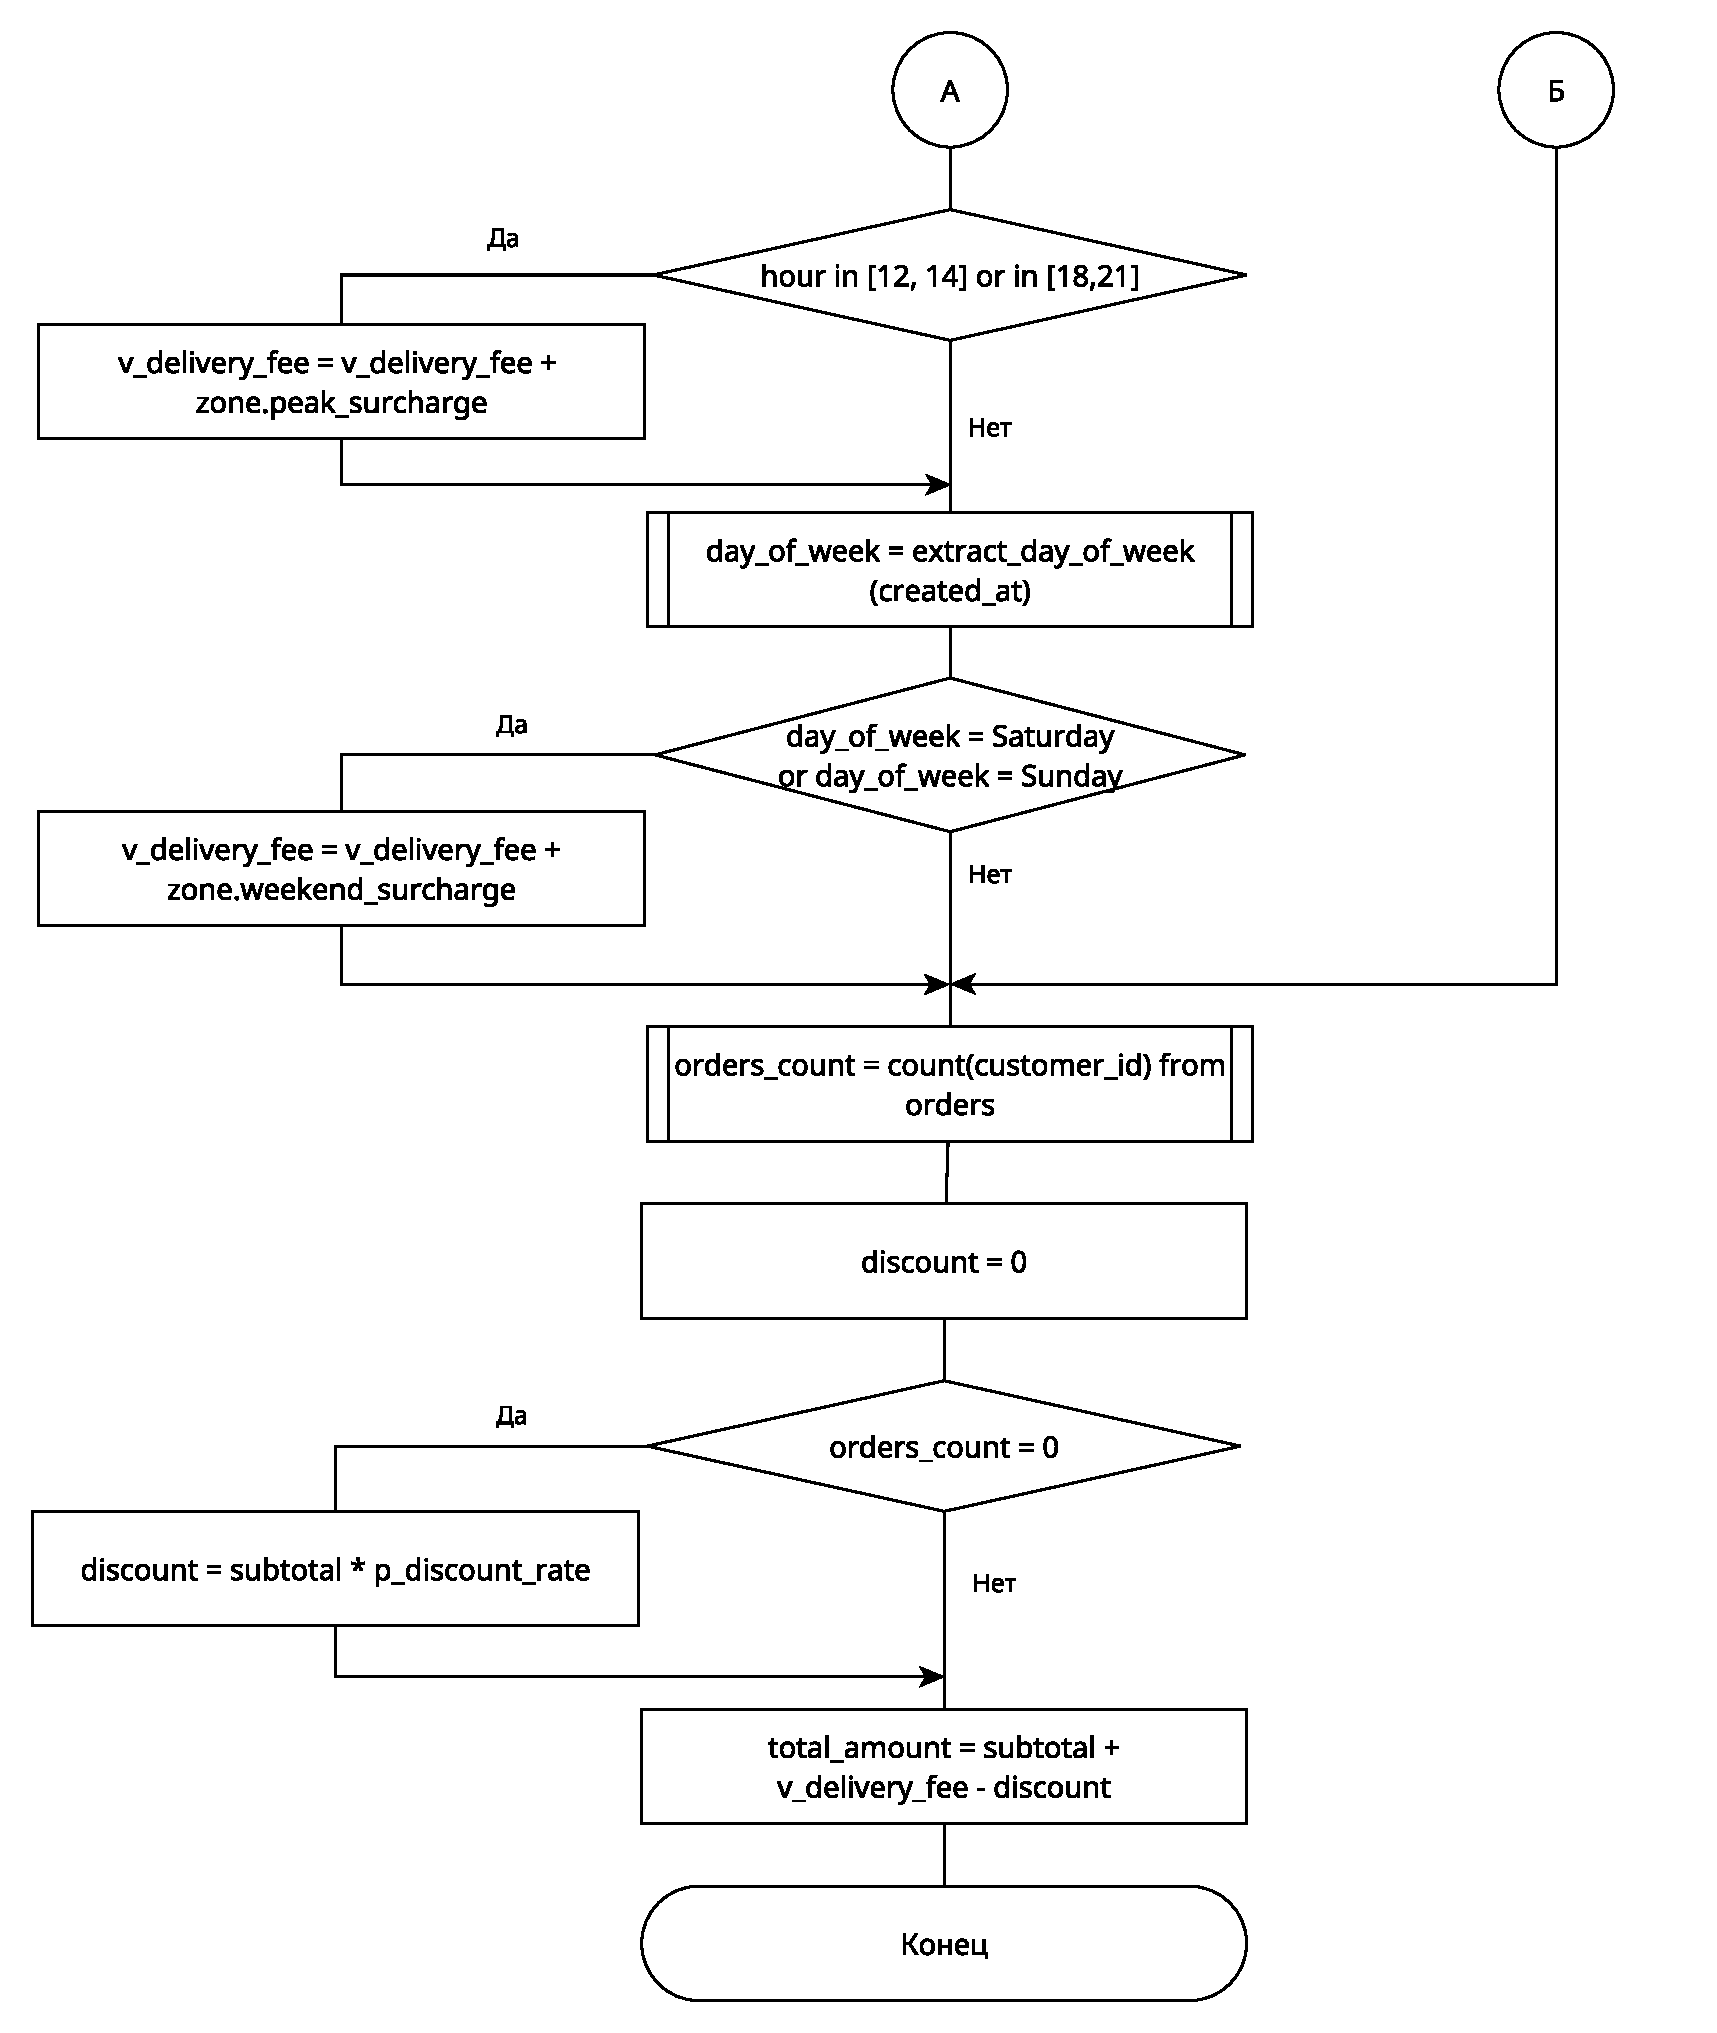
\includegraphics[scale=0.63]{img/function_2}}
		\caption{Функция подсчёта итоговой суммы заказа. Часть 2}
		\label{img:function_2}
\end{figure}

\subsection{Проектирование ролевой модели}

В соответствии с требованиями к системе разграничения доступа были спроектированы 
следующие роли: роль клиента, роль администратора ресторана, роль курьера 
и роль администратора системы.

Роль <<Клиент>> предназначена для пользователей, оформляющих заказы 
в системе. Данная роль имеет следующие права доступа:
\begin{itemize}
    \item чтение данных из таблиц \texttt{restaurants}, \texttt{dish\_categories} 
          и \texttt{dishes} для просмотра доступных ресторанов и меню;
    \item чтение и изменение собственных данных в таблице \texttt{customers};
    \item чтение, вставка и изменение собственных записей в таблице \\ \texttt{customer\_addresses} для управления адресами доставки;
    \item чтение и вставка записей в таблицу \texttt{orders} для создания новых 
          заказов (доступ ограничен только заказами данного клиента);
    \item чтение и вставка записей в таблицу \texttt{order\_items} для формирования 
          состава заказа;
    \item чтение данных из таблицы \texttt{payments} для просмотра информации 
          об оплате своих заказов;
    \item чтение, вставка и изменение собственных записей в таблице \\ \texttt{reviews} для оставления отзывов о заказах.
\end{itemize}

Роль <<Администратор ресторана>> предназначена для управления рестораном и его меню. Данная роль имеет следующие права доступа:
\begin{itemize}
    \item чтение и изменение данных в таблице \texttt{restaurants} для обновления 
          информации о своём ресторане;
    \item полный доступ (чтение, вставка, изменение, удаление) к таблицам \texttt{dish\_categories} и \texttt{dishes} для управления меню своего ресторана;
    \item чтение и изменение записей в таблице \texttt{orders} для обработки заказов своего ресторана;
    \item чтение данных из таблицы \texttt{order\_items} для просмотра состава заказов;
    \item чтение данных из таблицы \texttt{reviews} для анализа отзывов о своём ресторане.
\end{itemize}

Роль <<Курьер>> предназначена для сотрудников службы доставки. Данная роль имеет следующие права доступа:
\begin{itemize}
    \item чтение и изменение собственных данных в таблице \texttt{couriers};
    \item чтение и изменение записей в таблице \texttt{orders} для обновления статуса доставки назначенных ему заказов;
    \item чтение данных из таблицы \texttt{order\_items} для просмотра состава доставляемого заказа;
    \item чтение данных из таблиц \texttt{restaurants}, \texttt{customer\_addresses} и \\\texttt{customers}  для получения информации о точках отправления и назначения;
    \item чтение данных из таблицы \texttt{reviews} для просмотра оценок своей работы.
\end{itemize}


Роль <<Администратор системы>> предназначена для технических специалистов, обслуживающих систему. Данная роль имеет следующие права доступа:
\begin{itemize}
    \item полный доступ ко всем таблицам базы данных для администрирования и устранения технических проблем;
    \item права на выполнение всех хранимых функций и процедур;
    \item доступ к системным объектам базы данных.
\end{itemize}

\subsection{Проектирование приложения}

Архитектура приложения построена на основе многослойной модели, включающей уровень представления для взаимодействия с клиентскими приложениями, уровень бизнес-логики для реализации бизнес-правил и уровень доступа к данным для работы с базой данных.

На рисунке~\ref{img:components} представлена диаграмма компонентов проектируемого приложения.
\jimg{components}{Диаграмма компонентов  приложения}

\subsection{Вывод}
В конструкторской части были спроектированы базы данных и ограничения её целостности. Обосновано соответствие таблиц третьей нормальной форме (3НФ). Составлен алгоритм функции для расчёта итоговой суммы заказа с учётом скидок и наценок. Описана ролевая модель доступа на уровне базы данных и спроектировано приложение для взаимодействия с базой данных